\problemname{Quack}

\illustration{0.4}{lotsofducks.jpg}
\noindent
Harry loves his small yellow ducks from Kodsport and has recently acquired a large collection.  

\noindent
But unfortunately, some of them have disappeared! The ducks are hiding in tall grass along a line, and the grass is so high that Harry cannot see where they are located.

There are $N$ ducks hiding at integer positions within the range $[0, 10^9]$, where each position can contain at most one duck. The problem is that Harry doesn't know how many ducks have disappeared.

However, Harry is able to perform the following action up to $Q$ times:

\begin{itemize}
    \item \textbf{Quack from a position:} Harry can stand at an integer position on the line $[-10^9, 2 \cdot 10^9]$ and begin quacking.
    \begin{itemize}
        \item The duck closest to Harry will then quack back, allowing Harry to determine the position of that particular duck.
        \item If there are multiple ducks with the same distance to Harry, the duck with the lower position will quack back first. This implies that Harry can only determine the position of the duck with lower position.
        \item Note that the ducks do not move or disappear after Harry finds them; they stay at their positions until all ducks have been identified.
    \end{itemize}
\end{itemize}

Your task is to help Harry find all the ducks by determining the number of ducks hiding and providing the exact positions of these ducks.

\begin{figure}[h!]
  \centering
  
\includegraphics[width=0.5\textwidth]{sample2.png}
  \caption{The secret placement of the hidden ducks in example case 2.}
\end{figure}

\section*{Interaction}
This is an interactive problem where you can place Harry at an integer position within the range $[-10^9, 2 \cdot 10^9]$ up to $Q$ times. 
Note that both $N$ and $Q$ are secret numbers.

Your program starts by reading an integer $T$ ($1 \leq T \leq 6$), where $T$ is the number of the test group. 
The reason for providing $T$ in the input is to make it easier to receive partial points.

After that, you can start placing Harry at any integer position $x_h$ within the range $[-10^9, 2 \cdot 10^9]$. You make the query by printing 
$$? \; x_h$$

Your program will then read an integer $x_a$, which is the position of the closest duck. 

If your program does not exit, you may receive incorrect assessments like \texttt{Run-Time Error}.

You can place Harry up to $Q$ times. But once you have found all $N$ duck positions $x_1 \; x_2 \; x_3 \; \dots \; x_N$, you should print two lines. 
First, a line with an exclamation mark and the number $N$, the number of hidden ducks:
$$! \; N$$
Then, print a new line with $N$ integers, the positions of the $N$ ducks in any order:
$$x_1 \; x_2 \; x_3 \; \dots \; x_N$$

After that, your program should terminate, and no further output should be printed.    

It is guaranteed that the number of lost ducks $N$ and their positions in each test case are predetermined and do not change adaptively in response to your outputs.

Make sure to flush the output after \textbf{every print statement}, otherwise you may get a \textit{Time Limit Exceeded}.
In C++, this can be done for example with \texttt{cout << flush;} or \texttt{fflush(stdout);},
in Python this is done automatically when you use \texttt{input()}, but otherwise you need to use \texttt{sys.stdout.flush()},
and in Java with \texttt{System.out.flush();}.

Note also that if your program prints an invalid number or incorrect answer, it will be marked as \texttt{Wrong Answer}, unless something else happens before it affects your assessment. 

\section*{Scoring}
Your solution will be tested on a set of test groups, each worth a number of points. Each test group contains
a set of test cases. To get the points for a test group you need to solve all test cases in the test group.

\noindent
\begin{tabular}{| l | l | p{12cm} |}
  \hline
  \textbf{Group} & \textbf{Points} & \textbf{Constraints} \\ \hline
  $1$    & $5$        & $N = 2$, $Q = 3$\\ \hline
  $2$    & $16$       & Ducks are located at $s$, $s+1$, $s+2$, $\ldots$, $s+N-1$ for some integer $0 \leq s \leq 10^9$, $2 \leq N \leq 2 \cdot 10^4, Q = 2N-1$. \\ \hline
  $3$    & $14$       & $2 \leq N \leq 100$, $Q = N^2+ N $ \\ \hline
  $4$    & $19$       & $2 \leq N \leq 100$, $Q = 33N$ \\ \hline
  $5$    & $27$       & $2 \leq N \leq 10^3$, $Q = 2N-1$ \\ \hline
  $6$    & $19$       & $2 \leq N \leq 2 \cdot 10^4$, $Q = 2N-1$ \\ \hline 
\end{tabular}

\section*{Explanation of Sample 2}
According to the interaction, the program first places Harry at position $1$ and quacks. 
The program then receives information that the nearest duck to position $1$ is at position $0$.

\begin{figure}[h!]
  \centering
  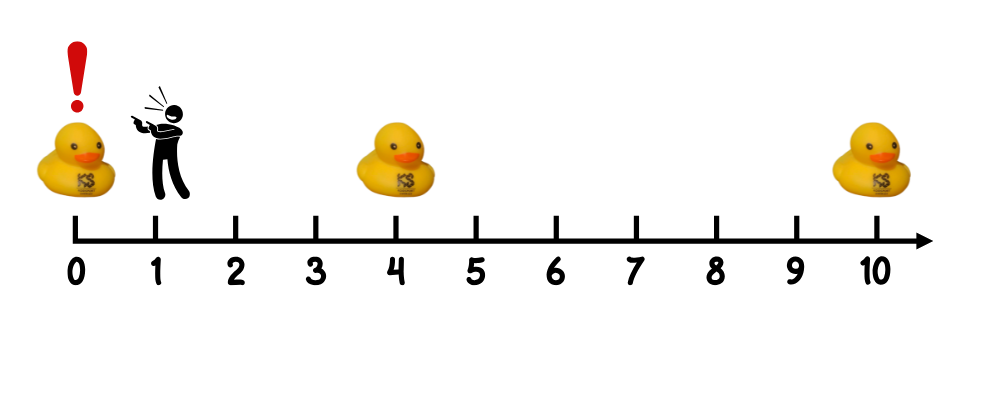
\includegraphics[width=0.5\textwidth]{sample2-p1.png}
\end{figure}

Then the program places Harry at position $4$ and quacks.
The program learns that the nearest duck to position $4$ is a duck at position $4$.
\begin{figure}[h!]
  \centering
  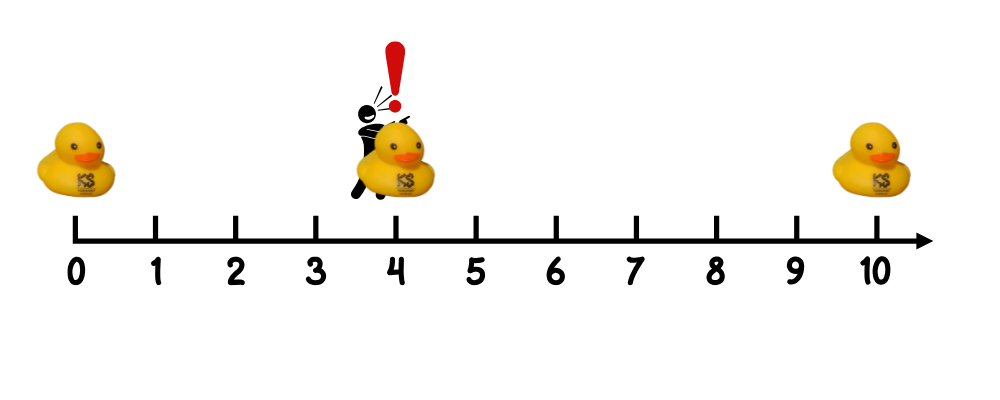
\includegraphics[width=0.5\textwidth]{sample2-p2.png}
\end{figure}

Next, the program places Harry at position $9$ and quacks.
The program receives information that the nearest duck to position $9$ is at position $10$.
\begin{figure}[h!]
  \centering
  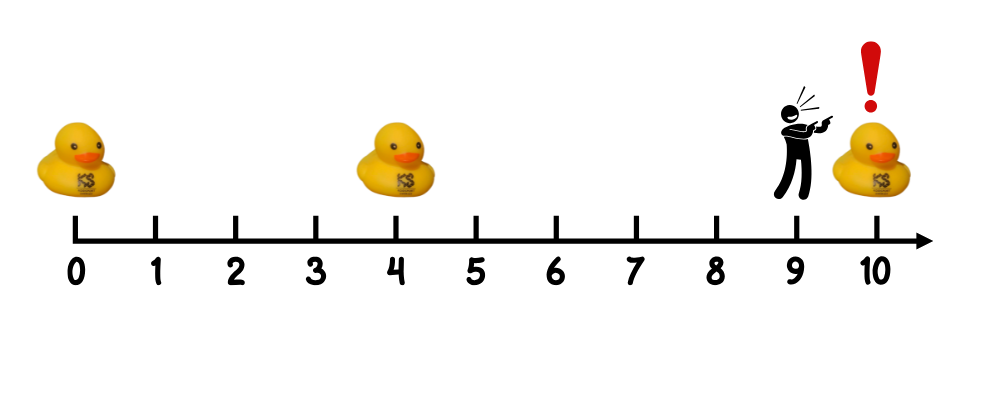
\includegraphics[width=0.5\textwidth]{sample2-p3.png}
\end{figure}

Then the program tries placing Harry at position $2$ and quacks.
Note that there are two different ducks at the same distance from Harry in this case. However, the program will only know about the duck with the lower coordinate-position, in this case, the duck at position $0$. 
\begin{figure}[h!]
  \centering
  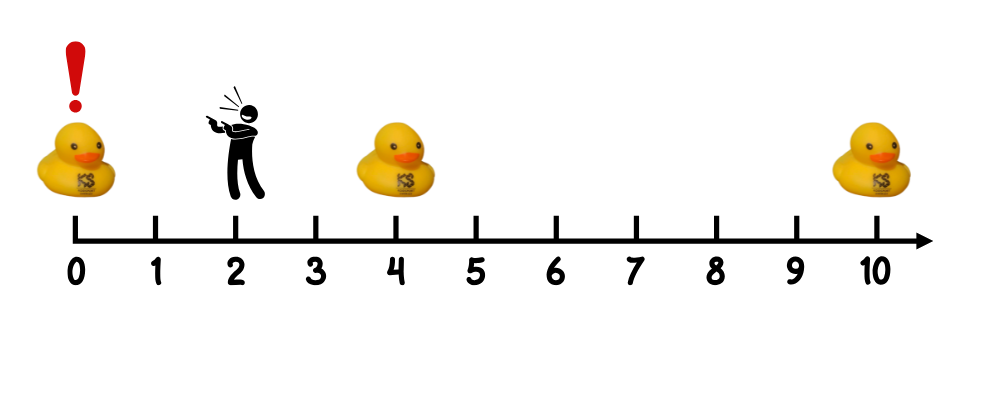
\includegraphics[width=0.5\textwidth]{sample2-p4.png}
\end{figure}

Finally, the program assumes that all ducks are found and prints the answer. 
